\section{Training der ML-Modelle}
\label{sec:model_training}
Typischerweise haben weder Entscheidungsbaum basierte Klassifizierer noch FFNNs Rückwärtskanten.
Neuronale Netze mit Rückwärtskanten werden als \textit{rekurrente Netze} (RNN) bezeichnet.
Abbildung \ref{fig:model_idea} zeigt, dass die Rückwärtskante genutzt wird, um das Klassifizierungsergebnis,
also den vorherigen Standort, bei der Feature-Extrahierung zu nutzen.
Das Klassifizierungsergebnis ist aber nicht immer korrekt, wodurch fehlerhafte Features im Zusammenhang
mit dem Klassifizierungsergebnis als Eingabe in das ML-Modell verwendet werden können.
Damit das ML-Modell lernt mit diesem Fehler umzugehen, ist es notwendig, dass das ML-Modell Trainingsbeispiele mit
Features auf Basis eigener Klassifizierungsbeispiele zur Verfügung hat.
\newline
\newline
Abbildung \ref{fig:training_explained} illustriert den Trainingsablauf.
Die simulierten Daten der aufgenommenen Routen sind unterteilt in Partitionen basierend auf deren Zyklusbeschriftung,
damit in jeder Partition alle Standorte vorhanden sind.
Der Zyklus ist ein Umlauf einer Route, bevor sie wiederholt wird.
Insgesamt besteht die Datenmenge aus 20 Zyklen.
Die ersten fünf Zyklen werden zum \glqq Aufwärmen \grqq\ verwendet,
d. h. das ML-Modell wird mit korrekt beschrifteten Daten trainiert, welche es nicht selbst beschriftet hat.
In den folgenden zehn Zyklen werden weitere Partitionen zur Trainingsmenge hinzugefügt, die mit quadratisch steigendem Anteil von dem ML-Modell selbst beschriftet sind.
Zunächst werden 50\% der Partition $i$ vom ML-Modell beschriftet, bis beim 13. Zyklus schließlich 100\% beschriftet wird.
Die Elemente aus der Partition, die beschriftet werden sollen, sind zufällig, damit der Klassifizierungsfehler auf allen Teilstücken der Route gelernt werden kann.
\begin{figure}[h!]
    \centering
    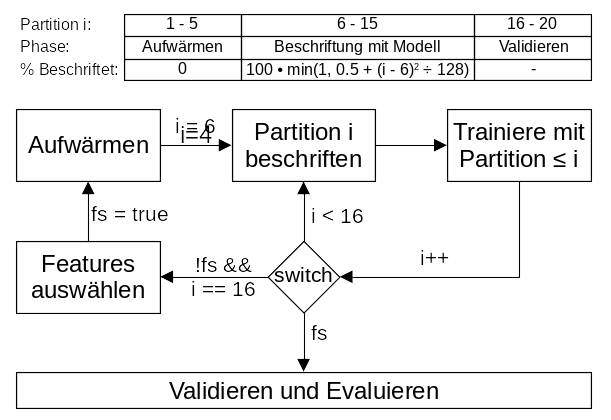
\includegraphics[width=\linewidth]{images/training_explained.png}
    \caption{Der Trainingsablauf des verfolgten Ansatzes.}
    \label{fig:training_explained}
\end{figure}
\newline
\newline
Die erste Trainingsphase ist abgeschlossen, nachdem das ML-Modell mit einer Trainingsmenge von 15 Zyklen trainiert wurde.
Anschließend wird einmalig eine Feature-Auswahl betrieben, in der insignifikante Features aus der Feature-Menge entfernt werden.
Insignifikante Features sind Feature, die eine geringe Wichtigkeit aufweisen (Kapitel \ref{sec:eval_feature_importance}).
Dies ermöglicht kleinere ML-Modelle zu verwenden und verringert die Dimensionen des Suchraumes, wodurch das Trainieren erleichtert wird.
Außerdem müssen Modelle individuell für verschiedene Einsatzgebiete trainiert werden, bei denen möglicherweise einige Sensoren bzw. Features nicht genutzt werden.
In Abbildung \ref{fig:training_explained} ist die Feature-Auswahl nur einmalig vorgesehen.
Denkbar wäre aber auch eine iterative Eliminierung der Features oder Optimierung durch ein evolutionären Algorithmus.
Anschließend wird das ML-Modell erneut auf den Partitionen trainiert, bis es validiert und evaluiert werden kann.
\newline
\newline
Die ML-Modelle ohne Rückwärtskante sind deutlich simpler.
Diese müssen nicht in Zyklen trainiert werden, sondern können direkt mit der vollständigen Trainingsmenge trainiert werden,
wodurch das Training deutlich effizienter ist.